\section[Architetture non von Neumann]{Architetture non von Neumann}
\label{sec:pipeline}
\sectionframe{images/covers/cover_pipeline.png}{Architetture \protect\linebreak non von Neumann}	 
 

\begin{frame}
	\frametitle{Aumentare le prestazioni delle CPU}

	\begin{block}{Aumentare le prestazioni delle CPU}
		Per potenziare le prestazioni delle CPU e dei sistemi di elaborazione, rimanendo ancorati ad una architettura di von Neumann, sono state prese in considerazione diverse strategie:
		\begin{itemize}
			\item l'incremento della frequenza di clock
			\item l'ampliamento della dimensione della parola
			\item l'aumento dello spazio di indirizzamento
		\end{itemize}
		
		Tuttavia, tutte queste strategie hanno raggiunto un punto limite nell'evoluzione delle architetture, oltre il quale ulteriori miglioramenti delle prestazioni sono diventati sempre più difficili.\\~\\
		
		Di conseguenza, è emersa un'altra prospettiva di sviluppo attraverso l'approccio di \textbf{architetture non von Neumann}.
	\end{block}

\end{frame}


\begin{frame}
	\frametitle{Aumentare le prestazioni delle CPU}

	\begin{figure}[!htbp]
		\centering
		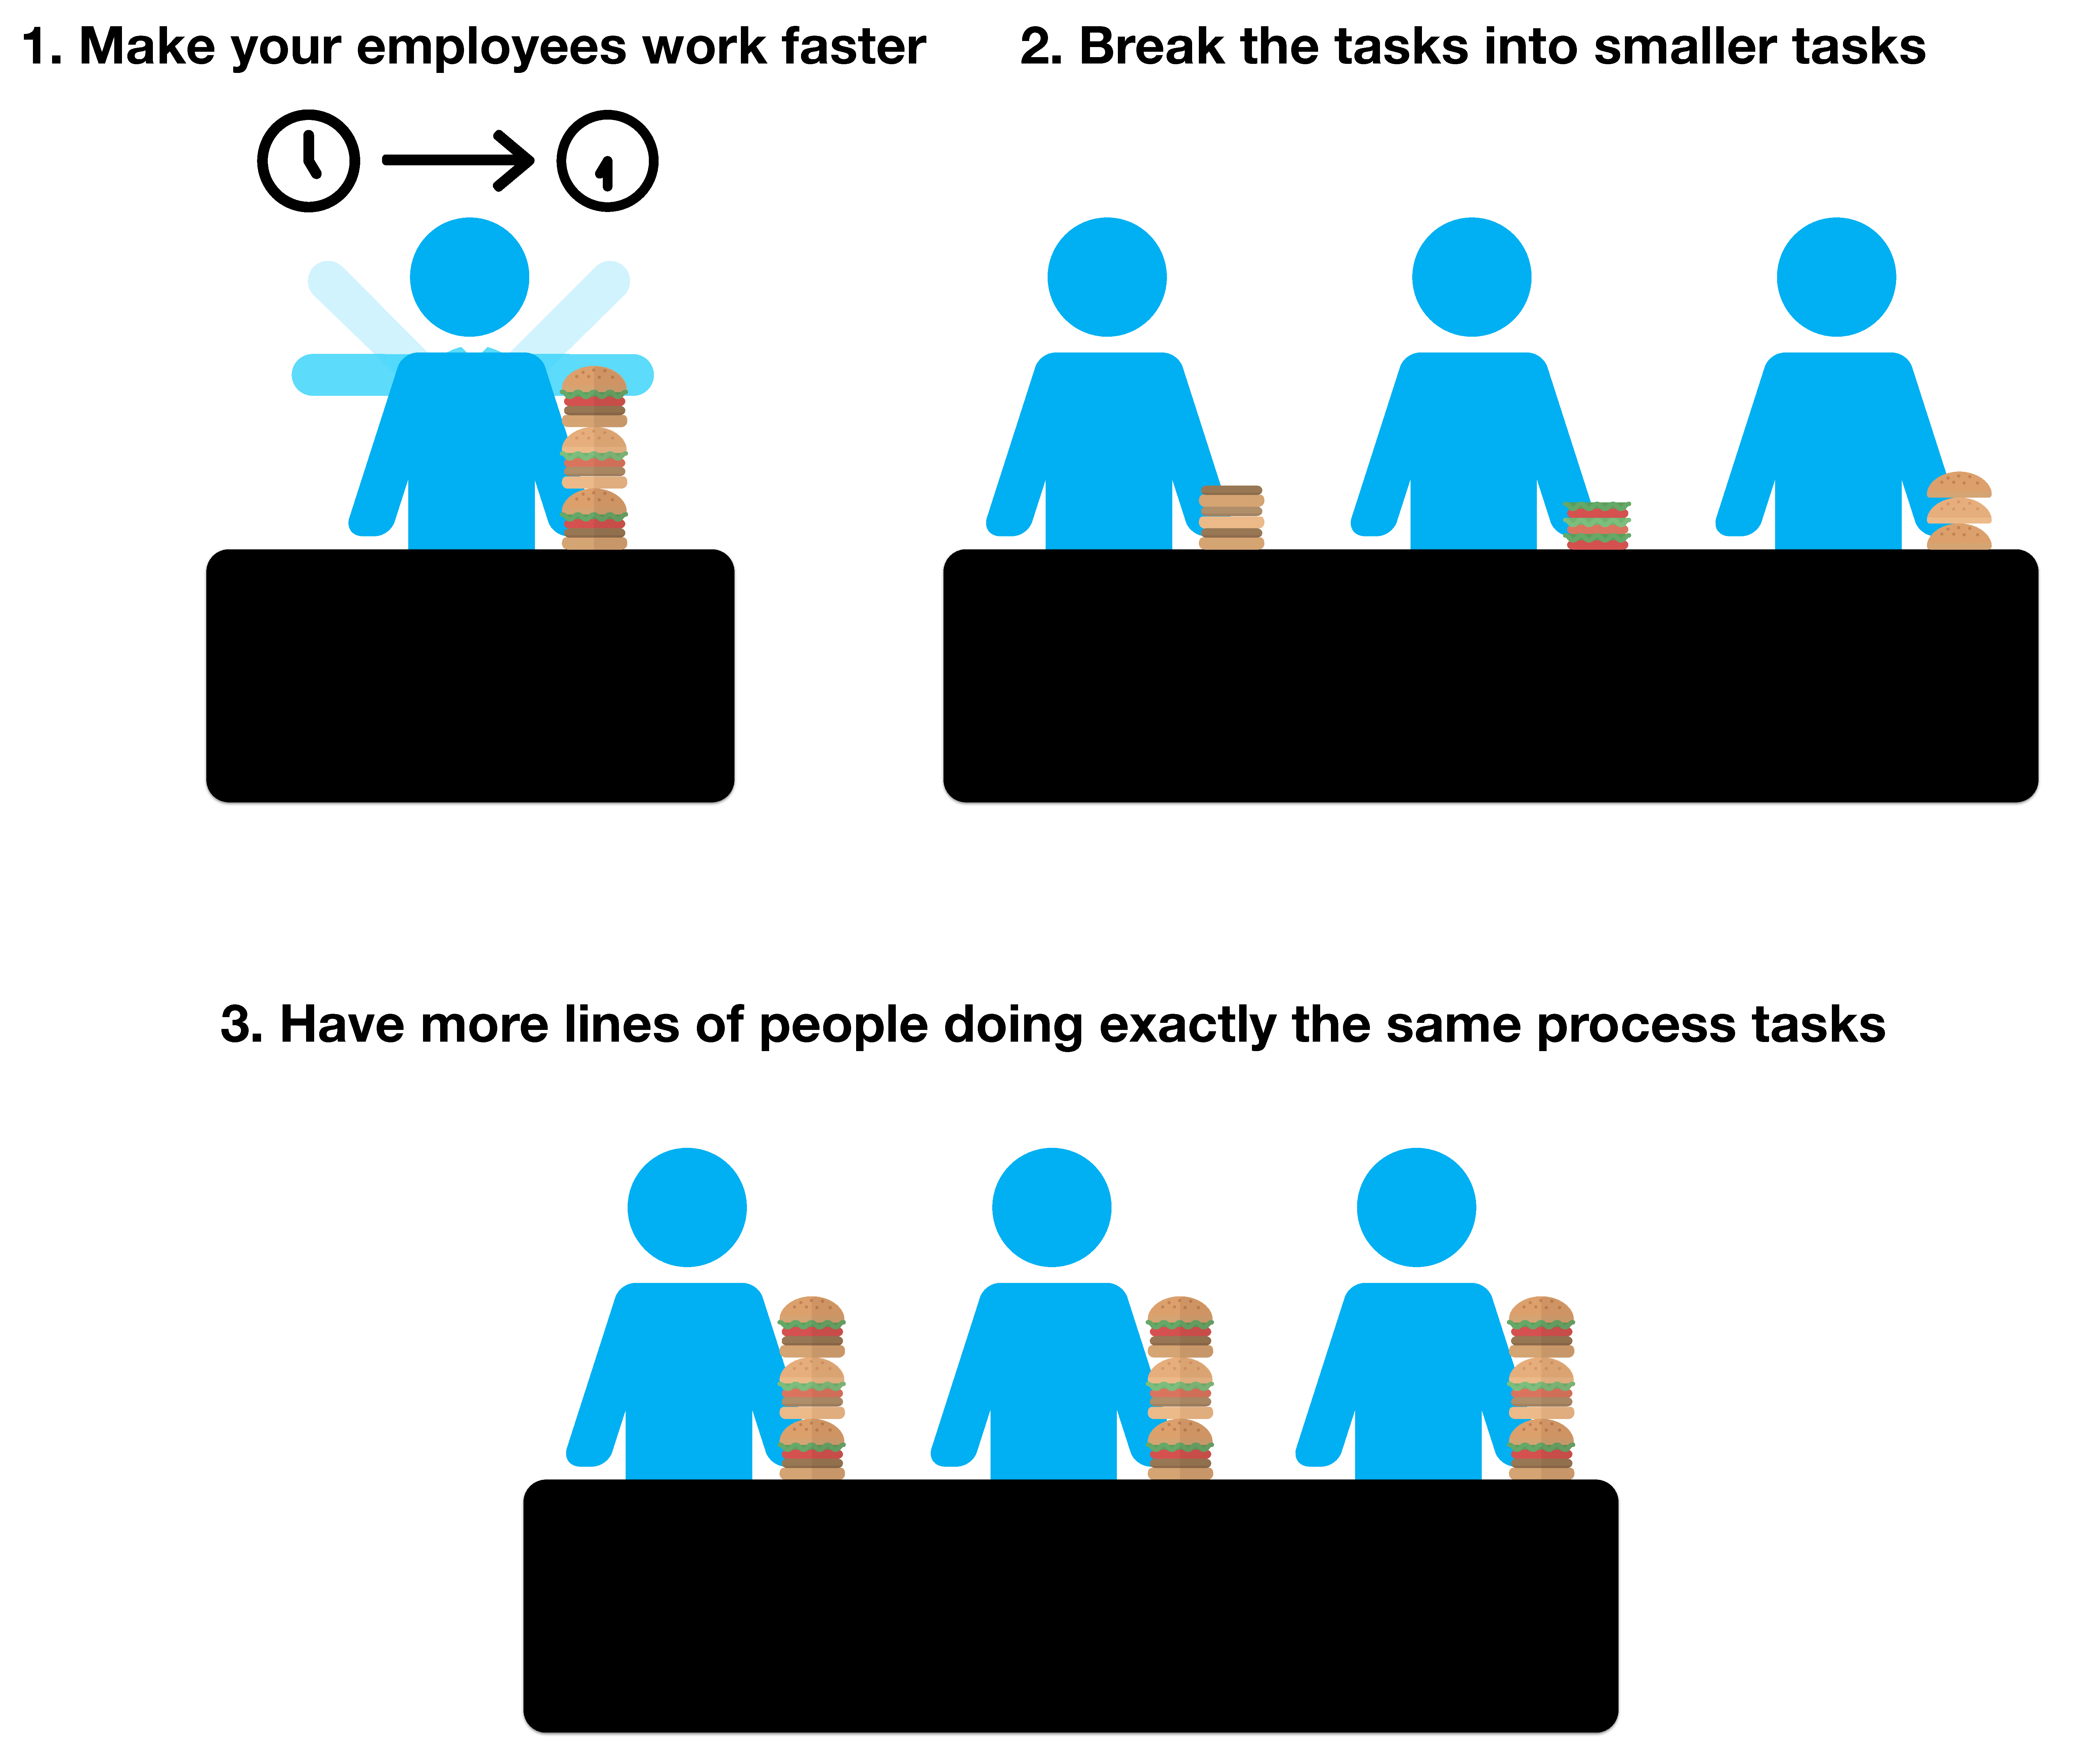
\includegraphics[width=0.73\linewidth]{images/7_pipeline/faster_cpu.pdf}
		%\caption{}
%		\label{}
	\end{figure}
\end{frame}


\begin{frame}
	\frametitle{Architetture non von Neumann}

	\begin{block}{Architetture non von Neumann}
		Elenchiamo alcune di questi possibili approcci:
		\begin{enumerate}
			\item Esecuzione fuori ordine
			\item Prefetch
			\item Speculative execution
			\item Pipeline
			\item Cache memory
			\item DMA (Direct Memory Access)
			\item Coprocessori
		\end{enumerate}
	\end{block}

\end{frame}


\subsection[Esecuzione fuori ordine]{Esecuzione fuori ordine}
\begin{frame}
	\frametitle{\textbullet{1} Esecuzione fuori ordine}

	%\begin{block}{Esecuzione fuori ordine}
		L'\textbf{esecuzione fuori ordine} è una tecnica avanzata utilizzata nelle CPU per migliorare l'efficienza nell'esecuzione delle istruzioni. Invece di eseguire le istruzioni nell'ordine in cui sono state ricevute, come accadeva nelle prime architetture, l'esecuzione fuori ordine permette alla CPU di eseguire istruzioni indipendenti in parallelo, sfruttando al massimo le risorse disponibili.\\~\\		
		Quando una CPU opera in modalità di esecuzione fuori ordine, può analizzare le istruzioni in entrata e identificare quelle che possono essere eseguite senza dipendenze da istruzioni precedenti. Queste istruzioni vengono inviate alle unità di esecuzione in parallelo, indipendentemente dall'ordine originale. Questo metodo \textbf{non sempre può essere impiegato}. Qualora due istruzioni consecutive siano dipendenti (ad esempio se la seconda istruzione usa il risultato ottenuto dalla prima istruzione) è necessario rispettare la sequenza operativa e le due istruzioni non potranno essere eseguite in parallelo.
	%\end{block}

\end{frame}


\begin{frame}
	\frametitle{\textbullet{1} Esecuzione fuori ordine}

	%\begin{block}{Esecuzione fuori ordine}
		L'esecuzione fuori ordine richiede hardware complesso, come buffer per riordinare i risultati in base all'ordine originale, unità di predizione delle dipendenze e logica per garantire l'integrità delle operazioni. Questa tecnica ha dimostrato di \textbf{migliorare notevolmente le prestazioni} delle CPU, consentendo loro di eseguire più istruzioni in modo parallelo e ottimizzato, pur mantenendo l'ordine corretto dei risultati in uscita.% \\~\\
		
		%
		
		\begin{figure}[!htbp]
			\centering 
			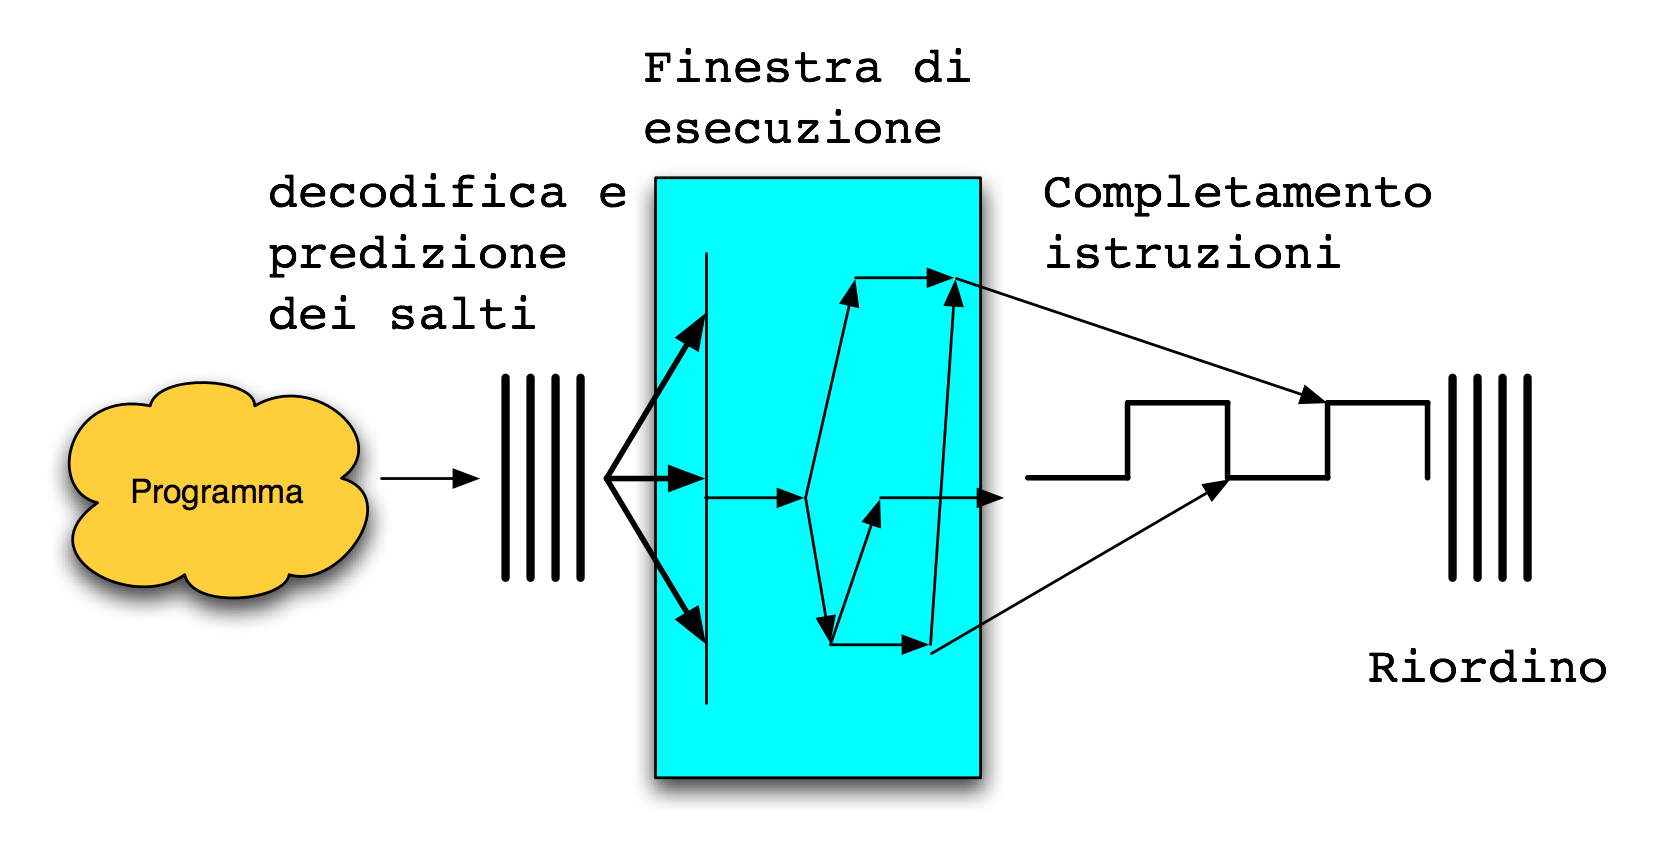
\includegraphics[width=0.7\linewidth]{images/7_pipeline/superscalar_processor.png}
			%\caption{}
			\label{fig:pipeline_superscalar_processor}
		\end{figure}
	%\end{block}

\end{frame}


\subsection[Prefetch]{Prefetch}
\begin{frame}
	\frametitle{\textbullet{2} Prefetch}

	%\begin{block}{Esecuzione fuori ordine}
		Nel contesto delle CPU, il \textbf{prefetch} è una tecnica di ottimizzazione che coinvolge il caricamento anticipato dei dati dalla memoria principale alla cache prima che siano effettivamente richiesti dall'esecuzione del programma. L'obiettivo principale del prefetch è ridurre i tempi di attesa e migliorare l'efficienza complessiva del sistema.\\~\\
		Il prefetch cerca di \textbf{prevedere quali dati saranno richiesti} successivamente e anticipa questo processo, caricando questi dati nella cache in modo che siano pronti per essere utilizzati quando verranno effettivamente richiesti. Questo può ridurre i ritardi dovuti all'accesso alla memoria, poiché i \textbf{dati richiesti sono già disponibili nella cache}, che è molto più veloce della memoria principale.
	%\end{block}

\end{frame}



\subsection[Speculative execution]{Speculative execution}
\begin{frame}
	\frametitle{\textbullet{3} Speculative execution}

	%\begin{block}{Esecuzione fuori ordine}
		La \textbf{speculative execution} (esecuzione speculativa) è una tecnica avanzata utilizzata nelle CPU per ottimizzare le prestazioni \textbf{eseguendo istruzioni} in \textbf{anticipo sulla base di previsioni}. Quando la CPU incontra un ramo condizionale (come un'istruzione di salto o un'istruzione condizionale), anziché attendere il risultato della condizione, la CPU esegue istruzioni speculativamente, seguendo la previsione più probabile.\\~\\
		\textbf{L'obiettivo della speculative execution è mitigare i ritardi causati dalle ramificazioni condizionali}. Se la previsione è corretta, l'esecuzione speculativa ha permesso alla CPU di eseguire istruzioni extra durante l'attesa della risposta condizionale. Tuttavia, se la previsione è errata, la CPU scarta semplicemente i risultati dell'esecuzione speculativa e riprende l'esecuzione dal punto corretto.\\
		Questa tecnica comporta l'utilizzo di unità di predizione dai branch per stimare quale sarà l'esito di una decisione condizionale.
	%\end{block}

\end{frame}


\subsection[Pipeline]{Pipeline}
\begin{frame}
	\frametitle{\textbullet{4} Pipeline}

	%\begin{block}{Esecuzione fuori ordine}
		La \textbf{pipeline} nei PC e nell'architettura dei processori si riferisce a una tecnica di progettazione che suddivide l'esecuzione di istruzioni in diversi \textbf{stadi sequenziali}. Ogni stadio rappresenta una parte del processo di esecuzione dell'istruzione, come il prelievo dell'istruzione dalla memoria, la decodifica dell'istruzione, l'esecuzione dell'istruzione e la scrittura dei risultati (rispettivamente fetch, decode, execute e write-back).\\~\\
		Questa suddivisione consente al processore di eseguire istruzioni in modo più efficiente e parallelo. Mentre un'istruzione è in fase di decodifica, il processore può iniziare a elaborare la successiva istruzione. Questo approccio riduce il tempo in cui il processore deve attendere che un'istruzione si completi prima di iniziare la successiva, aumentando così l'utilizzo delle risorse del processore.
	%\end{block}

\end{frame}


\begin{frame}
	\frametitle{\textbullet{4} Pipeline: laundry analogy}

	%\begin{block}{Esecuzione fuori ordine}
				
		\begin{figure}[!htbp]
			\centering 
			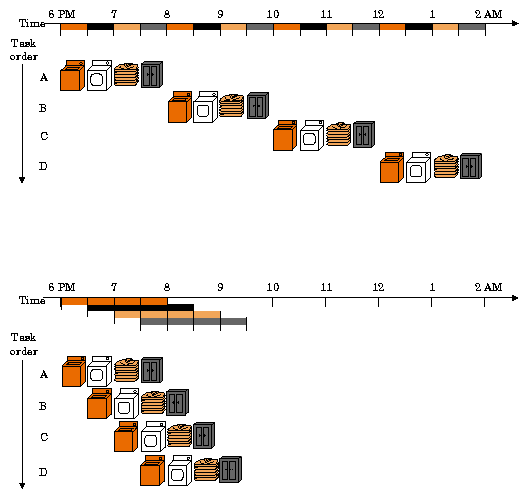
\includegraphics[width=0.5\linewidth]{images/7_pipeline/laundry_analogy.png}
			\caption{\textbf{Washer} takes 30 minutes, \textbf{Dryer} takes 30 minutes, \textbf{Folder} takes 30 minutes and \textbf{Stasher} takes 30 minutes: without pipeline to execute A, B, C, D tasks you would need 8 hours, with pipeline just 3.5 hours.}
			%\label{}
		\end{figure}
	%\end{block}

\end{frame}


% https://en.wikibooks.org/wiki/Microprocessor_Design/Pipelined_Processors
% https://en.wikipedia.org/wiki/Instruction_pipelining

\begin{frame}
	\frametitle{\textbullet{4} Pipeline}

	%\begin{block}{Esecuzione fuori ordine}
		Il numero di stadi varia in base all'architettura della macchina.\\
		La classica pipeline RISC comprende:
		\begin{itemize}
			\item Instruction fetch
			\item Instruction decode and register fetch
			\item Execute
			\item Memory access
			\item Register write back
		\end{itemize}
		
		Più una pipeline è \textit{profonda} (con un numero maggiore di stadi), più una specifico stadio può essere implementato con una circuiteria più semplice. Tali pipeline possono essere chiamate \textit{superpipeline}.\\
		Si dice che un processore è \textbf{fully pipelined} se è in grado di recuperare un'istruzione ad ogni ciclo. Pertanto, se alcune istruzioni o condizioni richiedono ritardi che inibiscono il recupero di nuove istruzioni, il processore non è \textit{fully pipelined}.
	%\end{block}

\end{frame}


\subsubsection[MIPS (Microprocessor without Interlocked Pipelined Stages)]{MIPS (Microprocessor without Interlocked Pipelined Stages)}
\begin{frame}
	\frametitle{\textbullet{4} Pipeline}

	%\begin{block}{Esecuzione fuori ordine}
		Gli stadi della classica pipeline RISC:
		\begin{itemize}
			\item \textbf{Instruction fetch (IF)}:\\ lettura dell'istruzione dalla memoria
			\item \textbf{Instruction decode and register fetch (ID)}:\\ decodifica dell'istruzione e lettura degli operandi da registri
			\item \textbf{Execute (EX)}:\\ esecuzione dell’istruzione
			\item \textbf{Memory access (MEM)}:\\ attivazione della memoria
			\item \textbf{Register write back (WB)}:\\ scrittura del risultato nel registro opportuno
		\end{itemize}
		
		\begin{figure}[!htbp]
			\centering 
			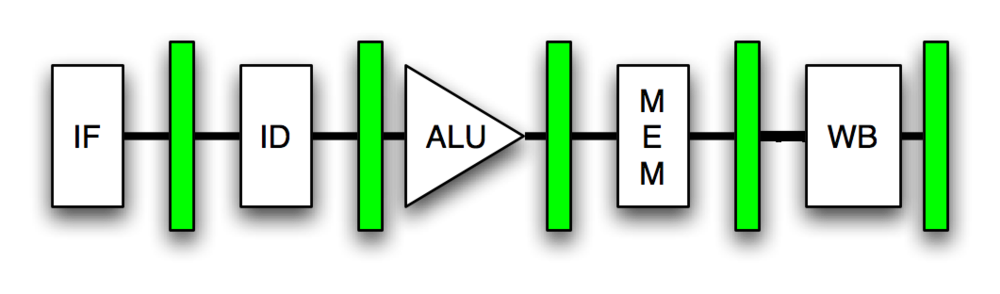
\includegraphics[width=0.63\linewidth]{images/7_pipeline/pipeline_base.png}
			%\caption{}
			\label{fig:pipeline_pipeline_base}
		\end{figure}
		
	%\end{block}

\end{frame}


\begin{frame}
	\frametitle{\textbullet{4} Pipeline}

	%\begin{block}{Esecuzione fuori ordine}
		\begin{figure}[!htbp]
			\centering 
			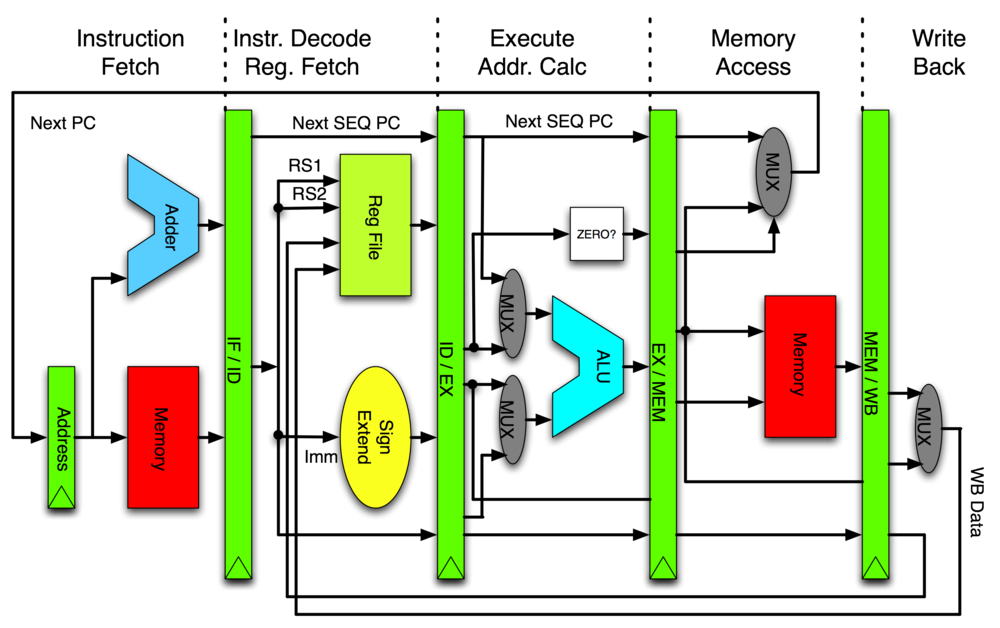
\includegraphics[width=0.82\linewidth]{images/7_pipeline/pipeline_mips_structure.png}
			\caption{Una architettura MIPS in 5 stadi}
			% (Microprocessor without Interlocked Pipelined Stages)
			\label{fig:pipeline_mips_structure}
		\end{figure}
	%\end{block}

\end{frame}


\begin{frame}
	\frametitle{\textbullet{4} Pipeline}

	%\begin{block}{Esecuzione fuori ordine}
		\begin{figure}[!htbp]
			\centering 
			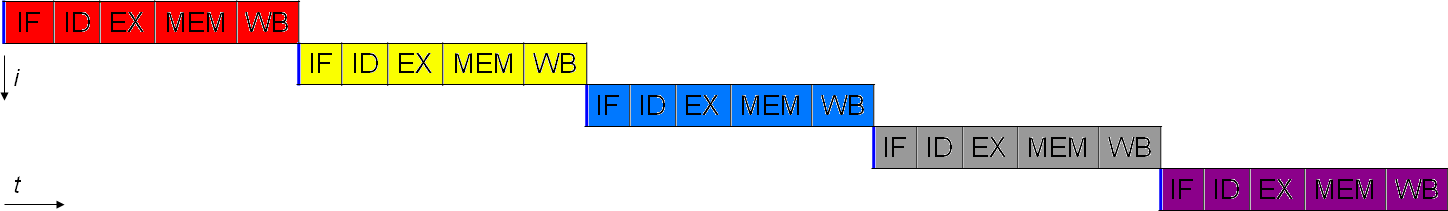
\includegraphics[width=1.0\linewidth]{images/7_pipeline/pipeline_no.png}
			\caption{Se eseguissi 5 istruzioni senza sfruttare la pipeline in ogni istante di tempo sarebbe presente una sola istruzione alla volta all'interno della pipeline.}
%			\label{}
		\end{figure}
	%\end{block}

\end{frame}


\begin{frame}
	\frametitle{\textbullet{4} Pipeline}

%	\begin{block}{Esecuzione fuori ordine}
%		\begin{columns}
%			\column{0.5\linewidth}
%			\begin{figure}[!htbp]
%				\centering 
%				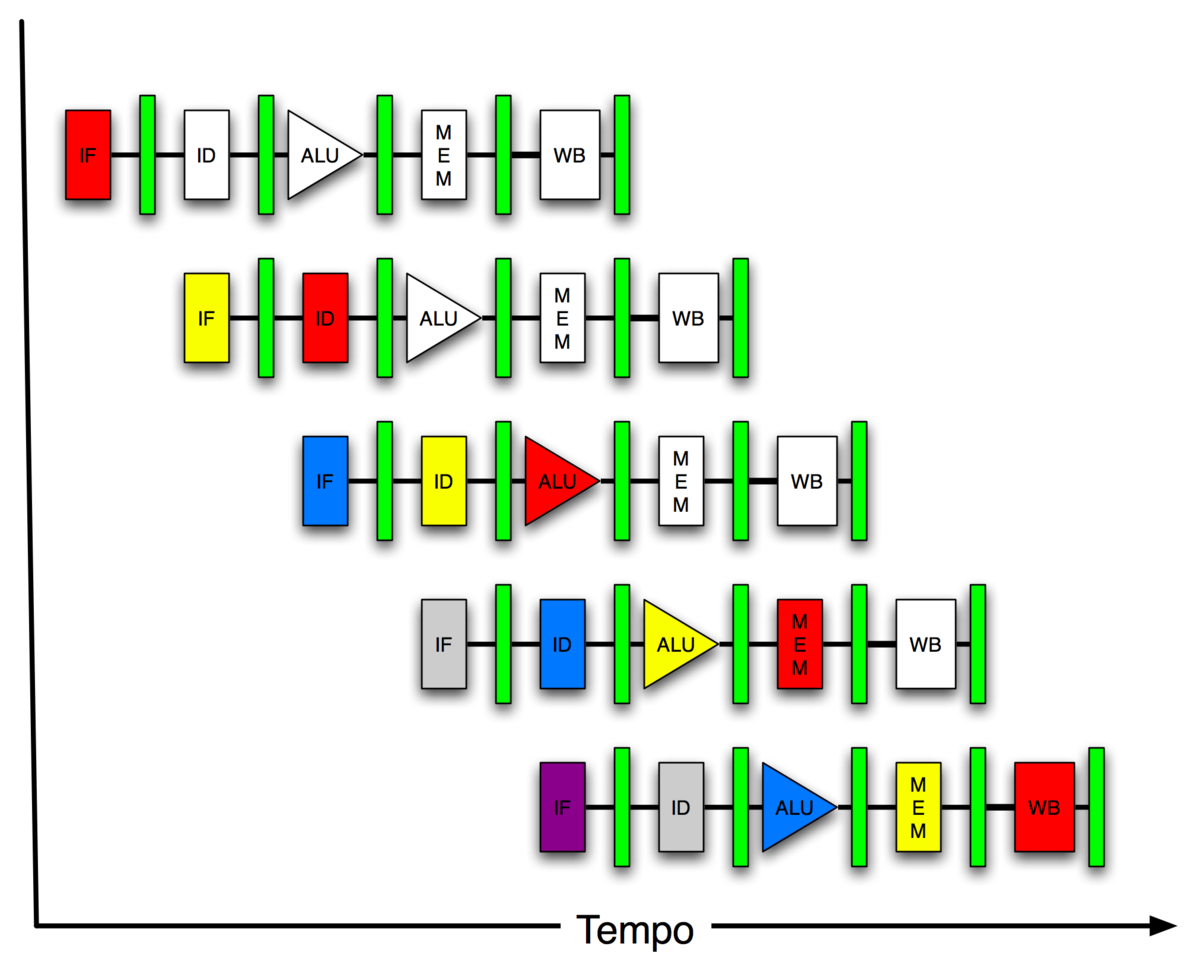
\includegraphics[width=1.0\linewidth]{images/7_pipeline/pipeline_in_time.png}
%				\caption{Se abbiamo 5 istruzioni, possiamo mostrarle nella nostra pipeline utilizzando colori diversi. Nel diagramma seguente, il bianco corrisponde a un NOP e i diversi colori corrispondono alle istruzioni nella pipeline. In ogni fase, le istruzioni avanzano attraverso la pipeline.}
%				\label{fig:pipeline_pipeline_in_time}
%			\end{figure}
%				
%			\column{0.5\linewidth}
%			\begin{figure}[!htbp]
%				\centering 
%				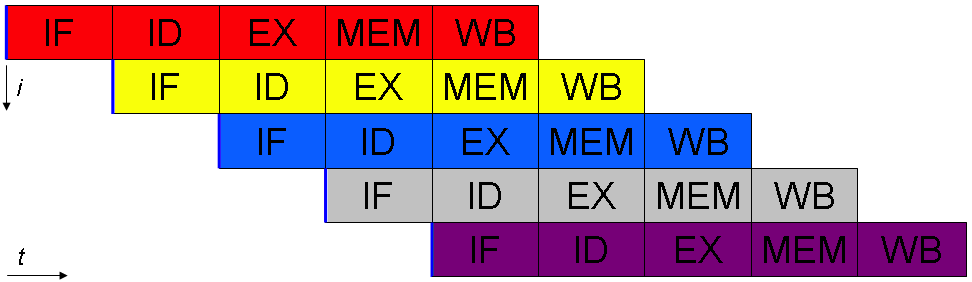
\includegraphics[width=1.0\linewidth]{images/7_pipeline/pipeline_five_stages.png}
%	%			\caption{}
%	%			\label{}
%			\end{figure}
%		\end{columns}
		
		
		\begin{figure}[htbp]
		    \centering
		    \begin{minipage}{0.49\textwidth}
		        \centering
		        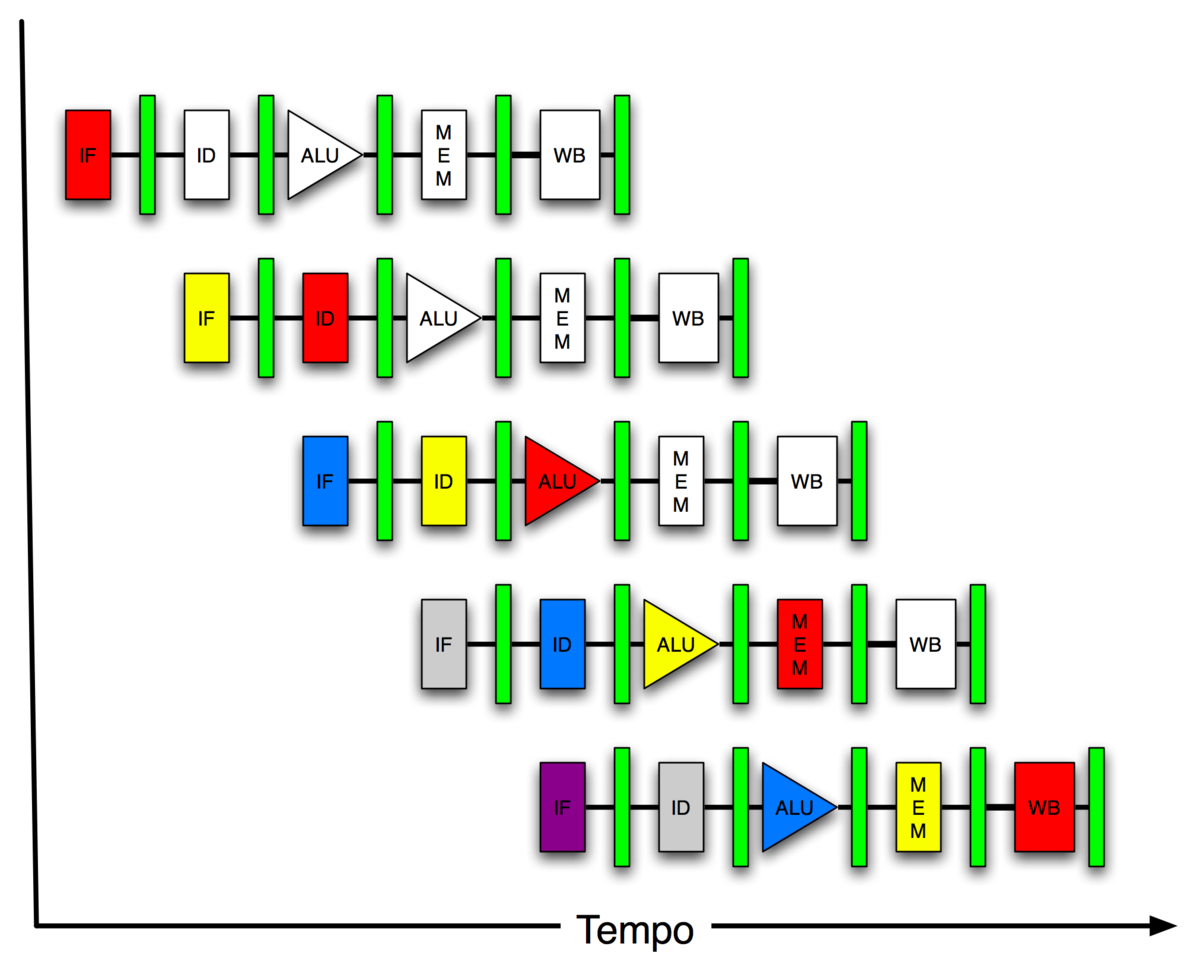
\includegraphics[width=1.0\linewidth]{images/7_pipeline/pipeline_in_time.png}
		        \label{fig:pipeline_pipeline_in_time}
		    \end{minipage}
		    \hfill
		    \begin{minipage}{0.49\textwidth}
		        \centering 
				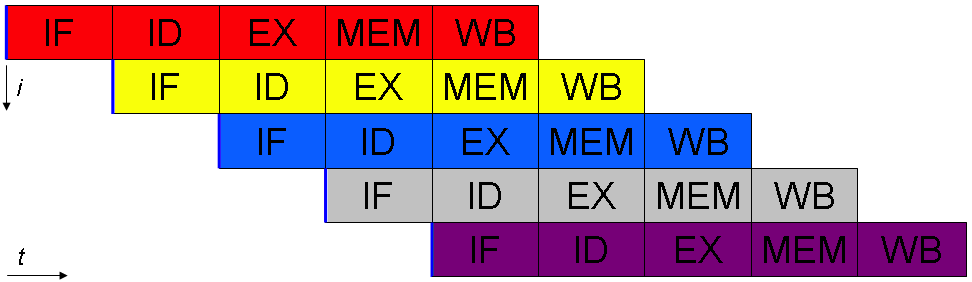
\includegraphics[width=1.0\linewidth]{images/7_pipeline/pipeline_five_stages.png}
		    \end{minipage}
		    \caption{Se abbiamo 5 istruzioni, possiamo mostrarle nella nostra pipeline utilizzando colori diversi. Nel diagramma seguente, il bianco corrisponde a un NOP e i diversi colori corrispondono alle istruzioni nella pipeline. In ogni stadio, le istruzioni avanzano attraverso la pipeline.}
		    \label{fig:pipeline_pipeline_in_time}
		\end{figure}
		
	%\end{block}

\end{frame}


\subsubsection[I conflitti]{I conflitti}
\begin{frame}
	\frametitle{\textbullet{4} Pipeline}

	%\begin{block}{Esecuzione fuori ordine}
		Tuttavia, la pipeline può incontrare situazioni in cui le istruzioni successive dipendono dai risultati di quelle precedenti. Chiamiamo tali situazioni problematiche \textbf{conflitti}.\\
		I conflitti possono essere causati da risorse limitate, dati mancanti o salti nell'esecuzione sequenziale delle istruzioni.\\~\\		
		Distinguiamo i tre principali tipi di conflitti:
		\begin{enumerate}
			\item \textbf{conflitti strutturali}: quando due stadi utilizzano contemporaneamente la stessa risorsa, come per esempio i BUS, l’ALU o la memoria RAM;
			\item \textbf{conflitti tra i dati}: quando un'istruzione utilizza un dato che è ancora in fase di elaborazione;
			\item \textbf{conflitti di controllo}: si verificano quando istruzioni di salto creano incertezza circa quale sia la successiva istruzione da andare effettivamente ad eseguire.
		\end{enumerate}
		
	%\end{block}
\end{frame}



\begin{frame}
	\frametitle{\textbullet{4} Pipeline}

	%\begin{block}{Esecuzione fuori ordine}
		\begin{figure}[!htbp]
			\centering 
			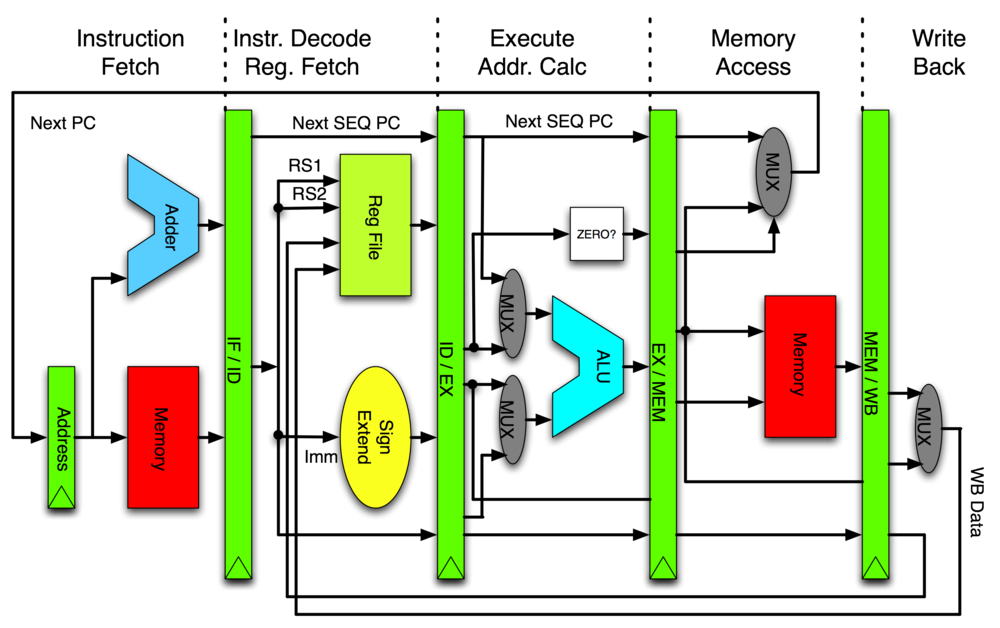
\includegraphics[width=0.82\linewidth]{images/7_pipeline/pipeline_mips_structure.png}
			\caption{Una architettura MIPS in 5 stadi}
			% (Microprocessor without Interlocked Pipelined Stages)
			\label{fig:pipeline_mips_structure}
		\end{figure}
	%\end{block}

\end{frame}


\subsubsection[I conflitti strutturali]{I conflitti strutturali}
\begin{frame}
	\frametitle{\textbullet{4} Pipeline}

	\begin{block}{Conflitti strutturali}
		I \textbf{conflitti strutturali} nascono quando la combinazione delle istruzioni presenti in una macchina è tale per cui stadi distinti della pipeline lineare richiedono contemporaneamente l’uso (esclusivo) delle medesime risorse.\\~\\
		Per ridurre al minimo le occorrenze dei conflitti strutturali le architetture delle pipeline MIPS sono strutturate in modo tale che nello stadio IF sia previsto uno specifico sommatore di 4 a PC, per evitare il conflitto per l’uso della ALU tra le istruzioni in IF e in EXE. Allo stesso modo la presenza di due memorie evita che lo stadio IF entri in conflitto con lo stadio ME.\\~\\
		In presenza di conflitto la soluzione più semplice consiste nell’arrestare la pipeline fino alla sua eliminazione, generando una situazione di \textbf{stallo}. L’aspetto negativo di questa soluzione è la \underline{degradazione delle prestazioni}.
	\end{block}
\end{frame}


\subsubsection[I conflitti tra dati]{I conflitti tra dati}
\begin{frame}
	\frametitle{\textbullet{4} Pipeline}

	\begin{block}{Conflitti tra dati}
		I \textbf{conflitti tra dati} si verificano quando una istruzione dipende dai dati prodotti da un'altra istruzione che deve ancora attraversare tutte le fasi della pipeline. Se un'istruzione successiva tenta di utilizzare dati non ancora disponibili a causa del ritardo di propagazione attraverso la pipeline, si verifica un conflitto tra i dati.\\~\\
		Questo può richiedere che l'\textbf{istruzione} successiva venga \textbf{fermata} temporaneamente.\\~\\
		Alternativamente si può ricorrere al \textbf{forwarding} dei dati oppure procedere a livello software a \textbf{riordinare le istruzioni} (operazione tipicamente effettuata dai compilatori moderni) per eliminare/minimizzare le dipendenze e di conseguenza l'occorrenza di tali conflitti.
	\end{block}
\end{frame}


\subsubsection[I conflitti di controllo]{I conflitti di controllo}
\begin{frame}
	\frametitle{\textbullet{4} Pipeline}

	\begin{block}{Conflitti di controllo}
		I \textbf{conflitti di controllo} si verificano quando le decisioni di salti condizionati nelle istruzioni non sono ancora state risolte quando l'istruzione successiva dovrebbe essere eseguita.\\~\\
		Questo può accadere quando si incontrano istruzioni di salto in una fase precedente della pipeline e non è ancora chiaro quale percorso di istruzioni verrà eseguito.\\~\\
		Un processore basato su architettura x86 incontra un salto condizionato mediamente ogni circa 6/7 istruzioni. Pertanto risulta rilevante cercare di prevedere correttamente la direzione data dai salti condizionati (\textbf{branch prediction}), in modo tale da caricare in anticipo il blocco di istruzioni corretto nella pipeline (mantenendola fully pipelined).
	\end{block}
\end{frame}


\subsubsection[Stallo, Bolle e NOP]{Stallo, Bolle e NOP}
\begin{frame}
	\frametitle{\textbullet{4} Pipeline}
	
	\begin{block}{Stallo, Bolle e NOP}
		Solitamente l'eliminazione un conflitto richiede necessariamente uno stallo. Effettuare uno stallo corrisponde ad inserire una bolla nella pipeline.\\~\\
		In alcune architetture, la fase di esecuzione della pipeline deve sempre eseguire un'azione ad ogni ciclo. In tal caso, la bolla viene implementata fornendo istruzioni NOP ("nessuna operazione") alla fase di esecuzione, finché la bolla non viene superata.
		\begin{columns}
			\column{0.5\linewidth}
			\begin{figure}[!htbp]
				\centering 
				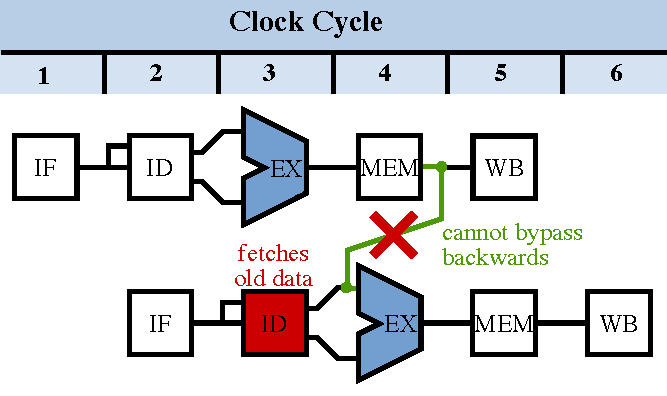
\includegraphics[width=0.75\linewidth]{images/7_pipeline/Data_Forwarding_(Two_Stage,_error).pdf}
				%\caption{Bypassing backwards in time	}
				\label{fig:pipeline_data_forwarding_error}
			\end{figure}
				
			\column{0.5\linewidth}
			\begin{figure}[!htbp]
				\centering 
				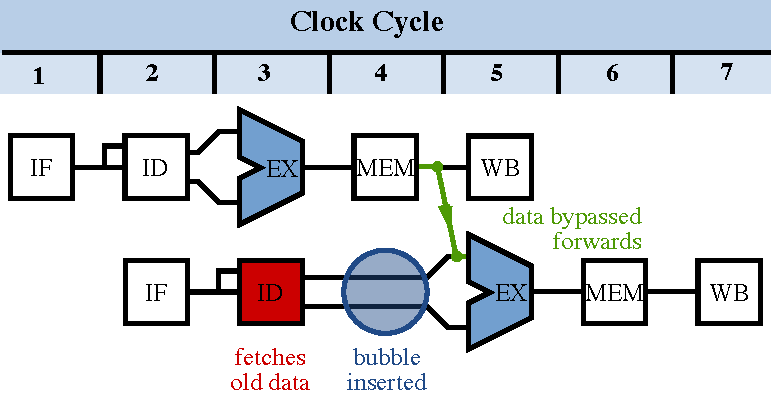
\includegraphics[width=0.85\linewidth]{images/7_pipeline/Data_Forwarding_(Two_Stage).pdf}
				%\caption{Problema risolto utilizzando una bolla e il forwarding}
				\label{fig:pipeline_data_forwarding_bubble}
			\end{figure}
		 \end{columns}
	 \end{block}
\end{frame}


\begin{frame}
	\frametitle{\textbullet{4} Pipeline}
	 
	\begin{columns}
		\column{0.5\linewidth}
		\begin{figure}[!htbp]
			\centering 
			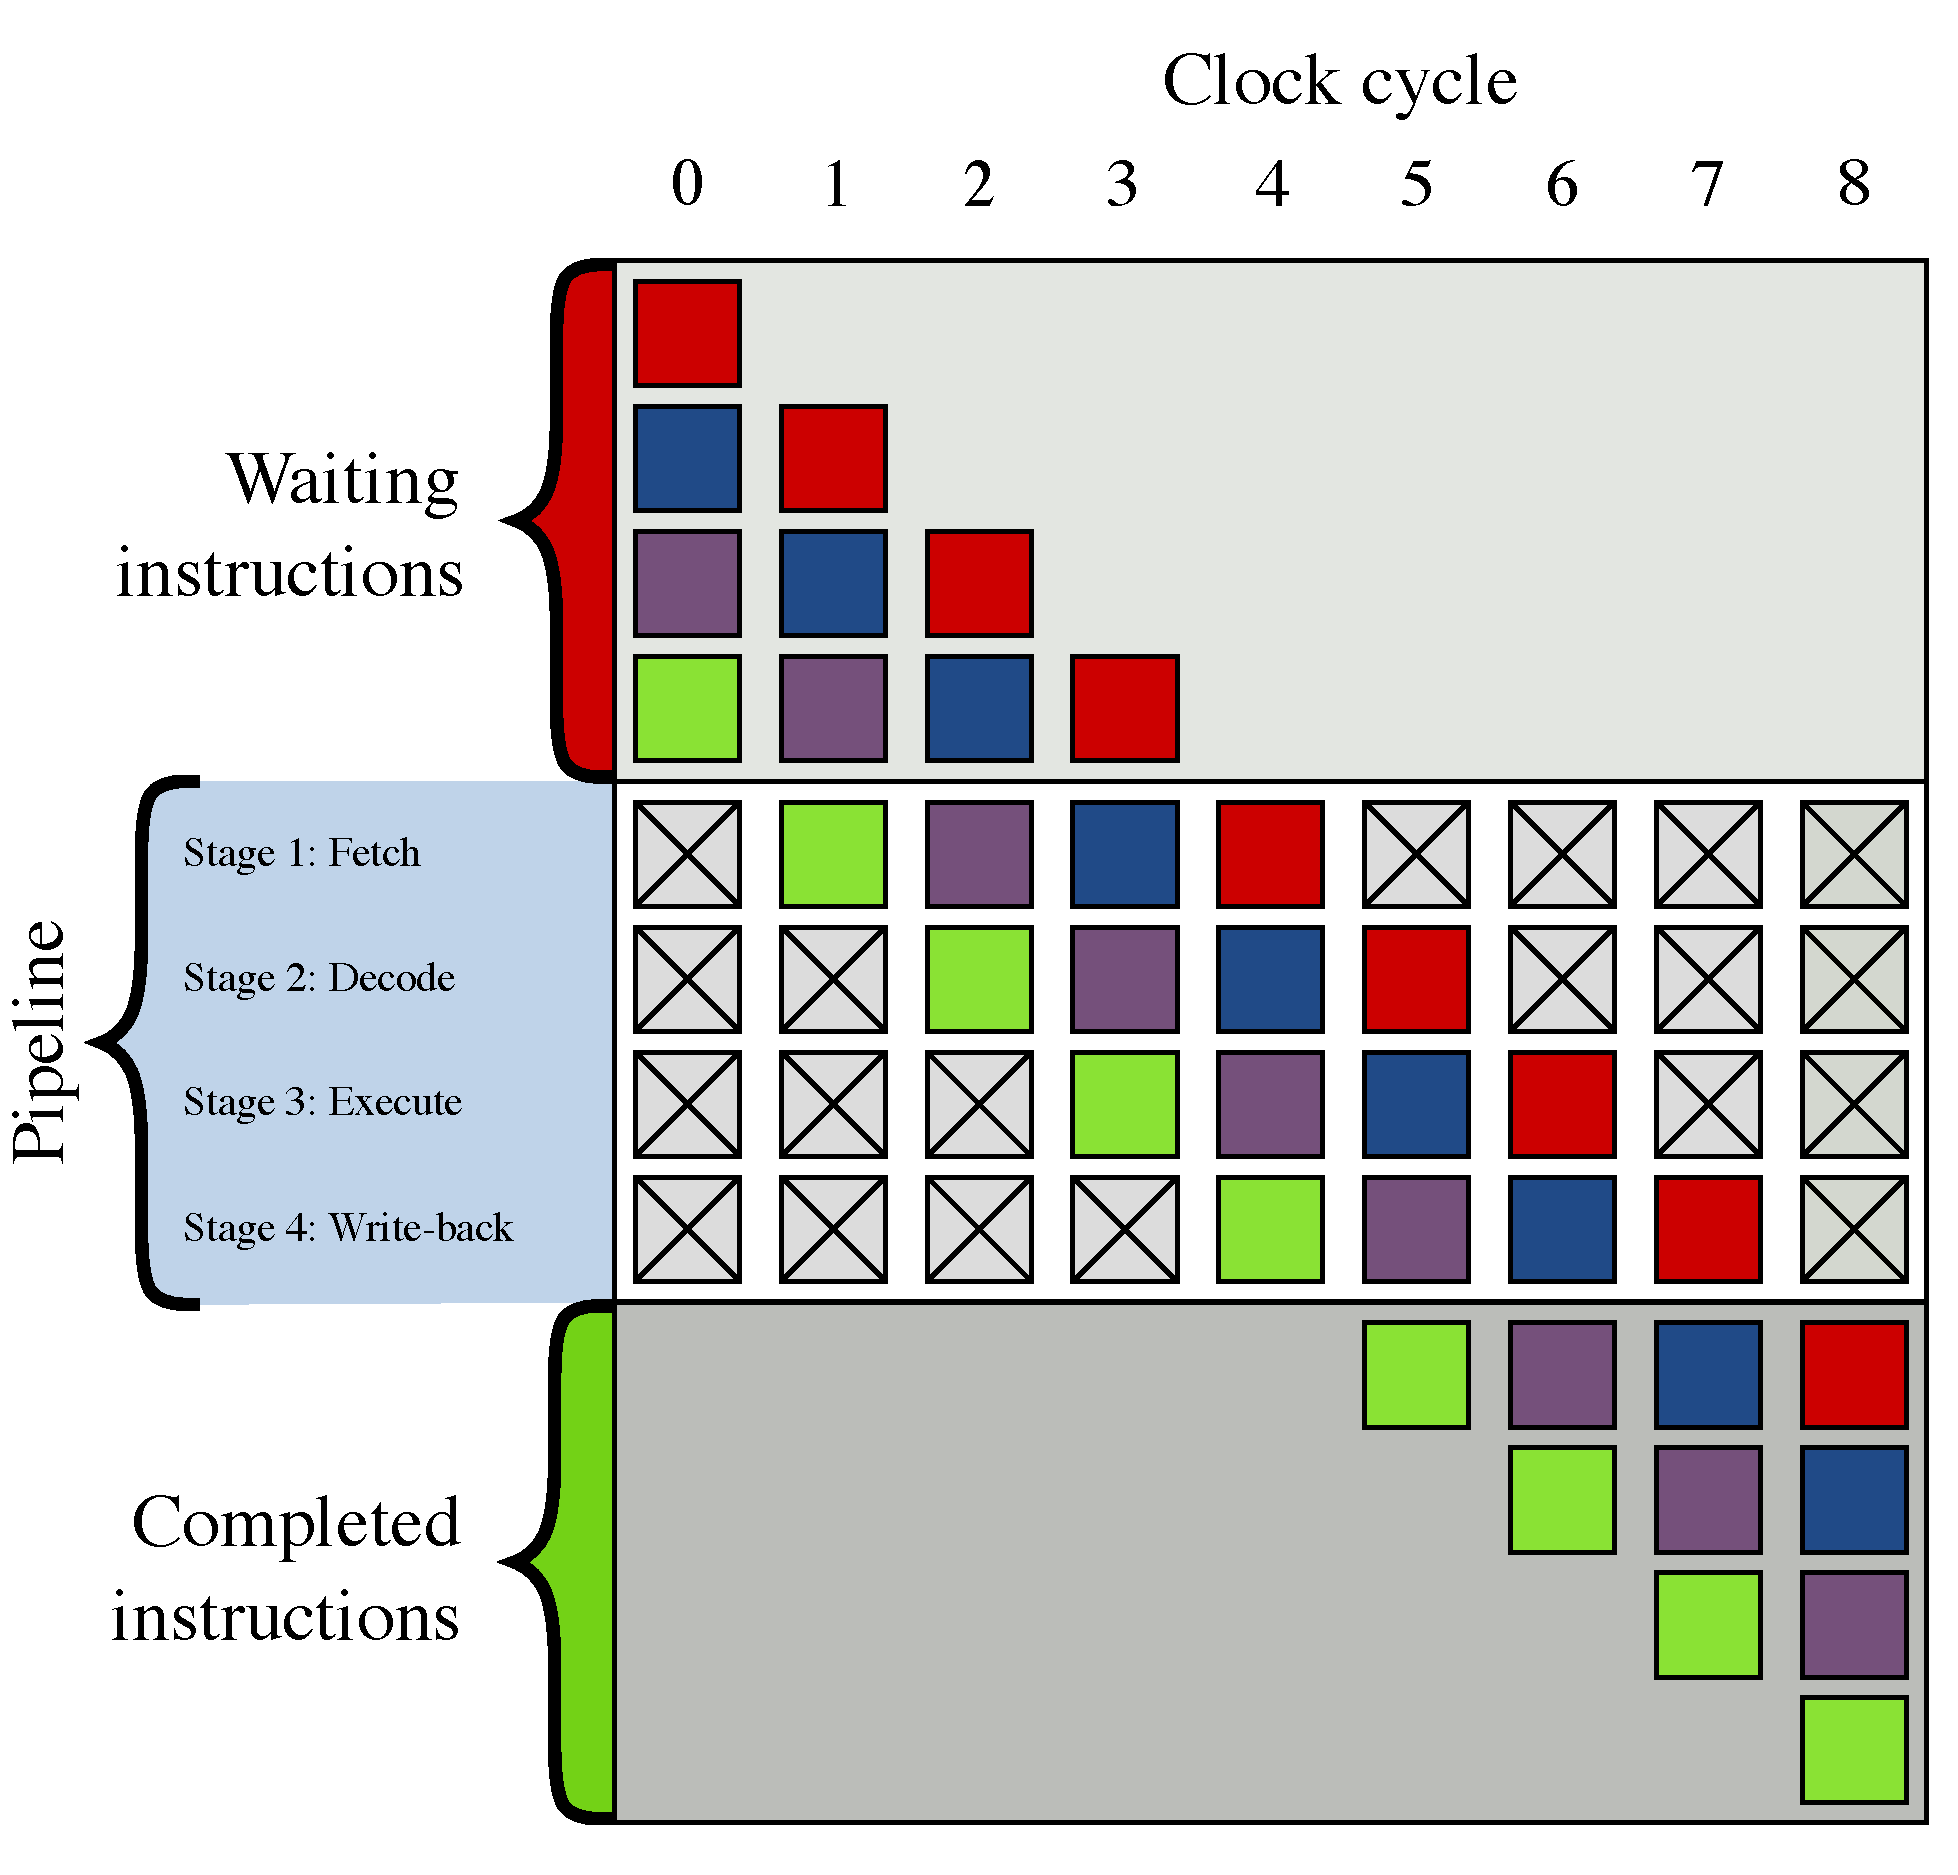
\includegraphics[width=1.0\linewidth]{images/7_pipeline/pipeline_4_stage.pdf}
			\caption{Esecuzione normale di una Pipeline in 4 stadi}
			\label{fig:pipeline_4_stage}
		\end{figure}
			
		\column{0.5\linewidth}
		\begin{figure}[!htbp]
			\centering 
			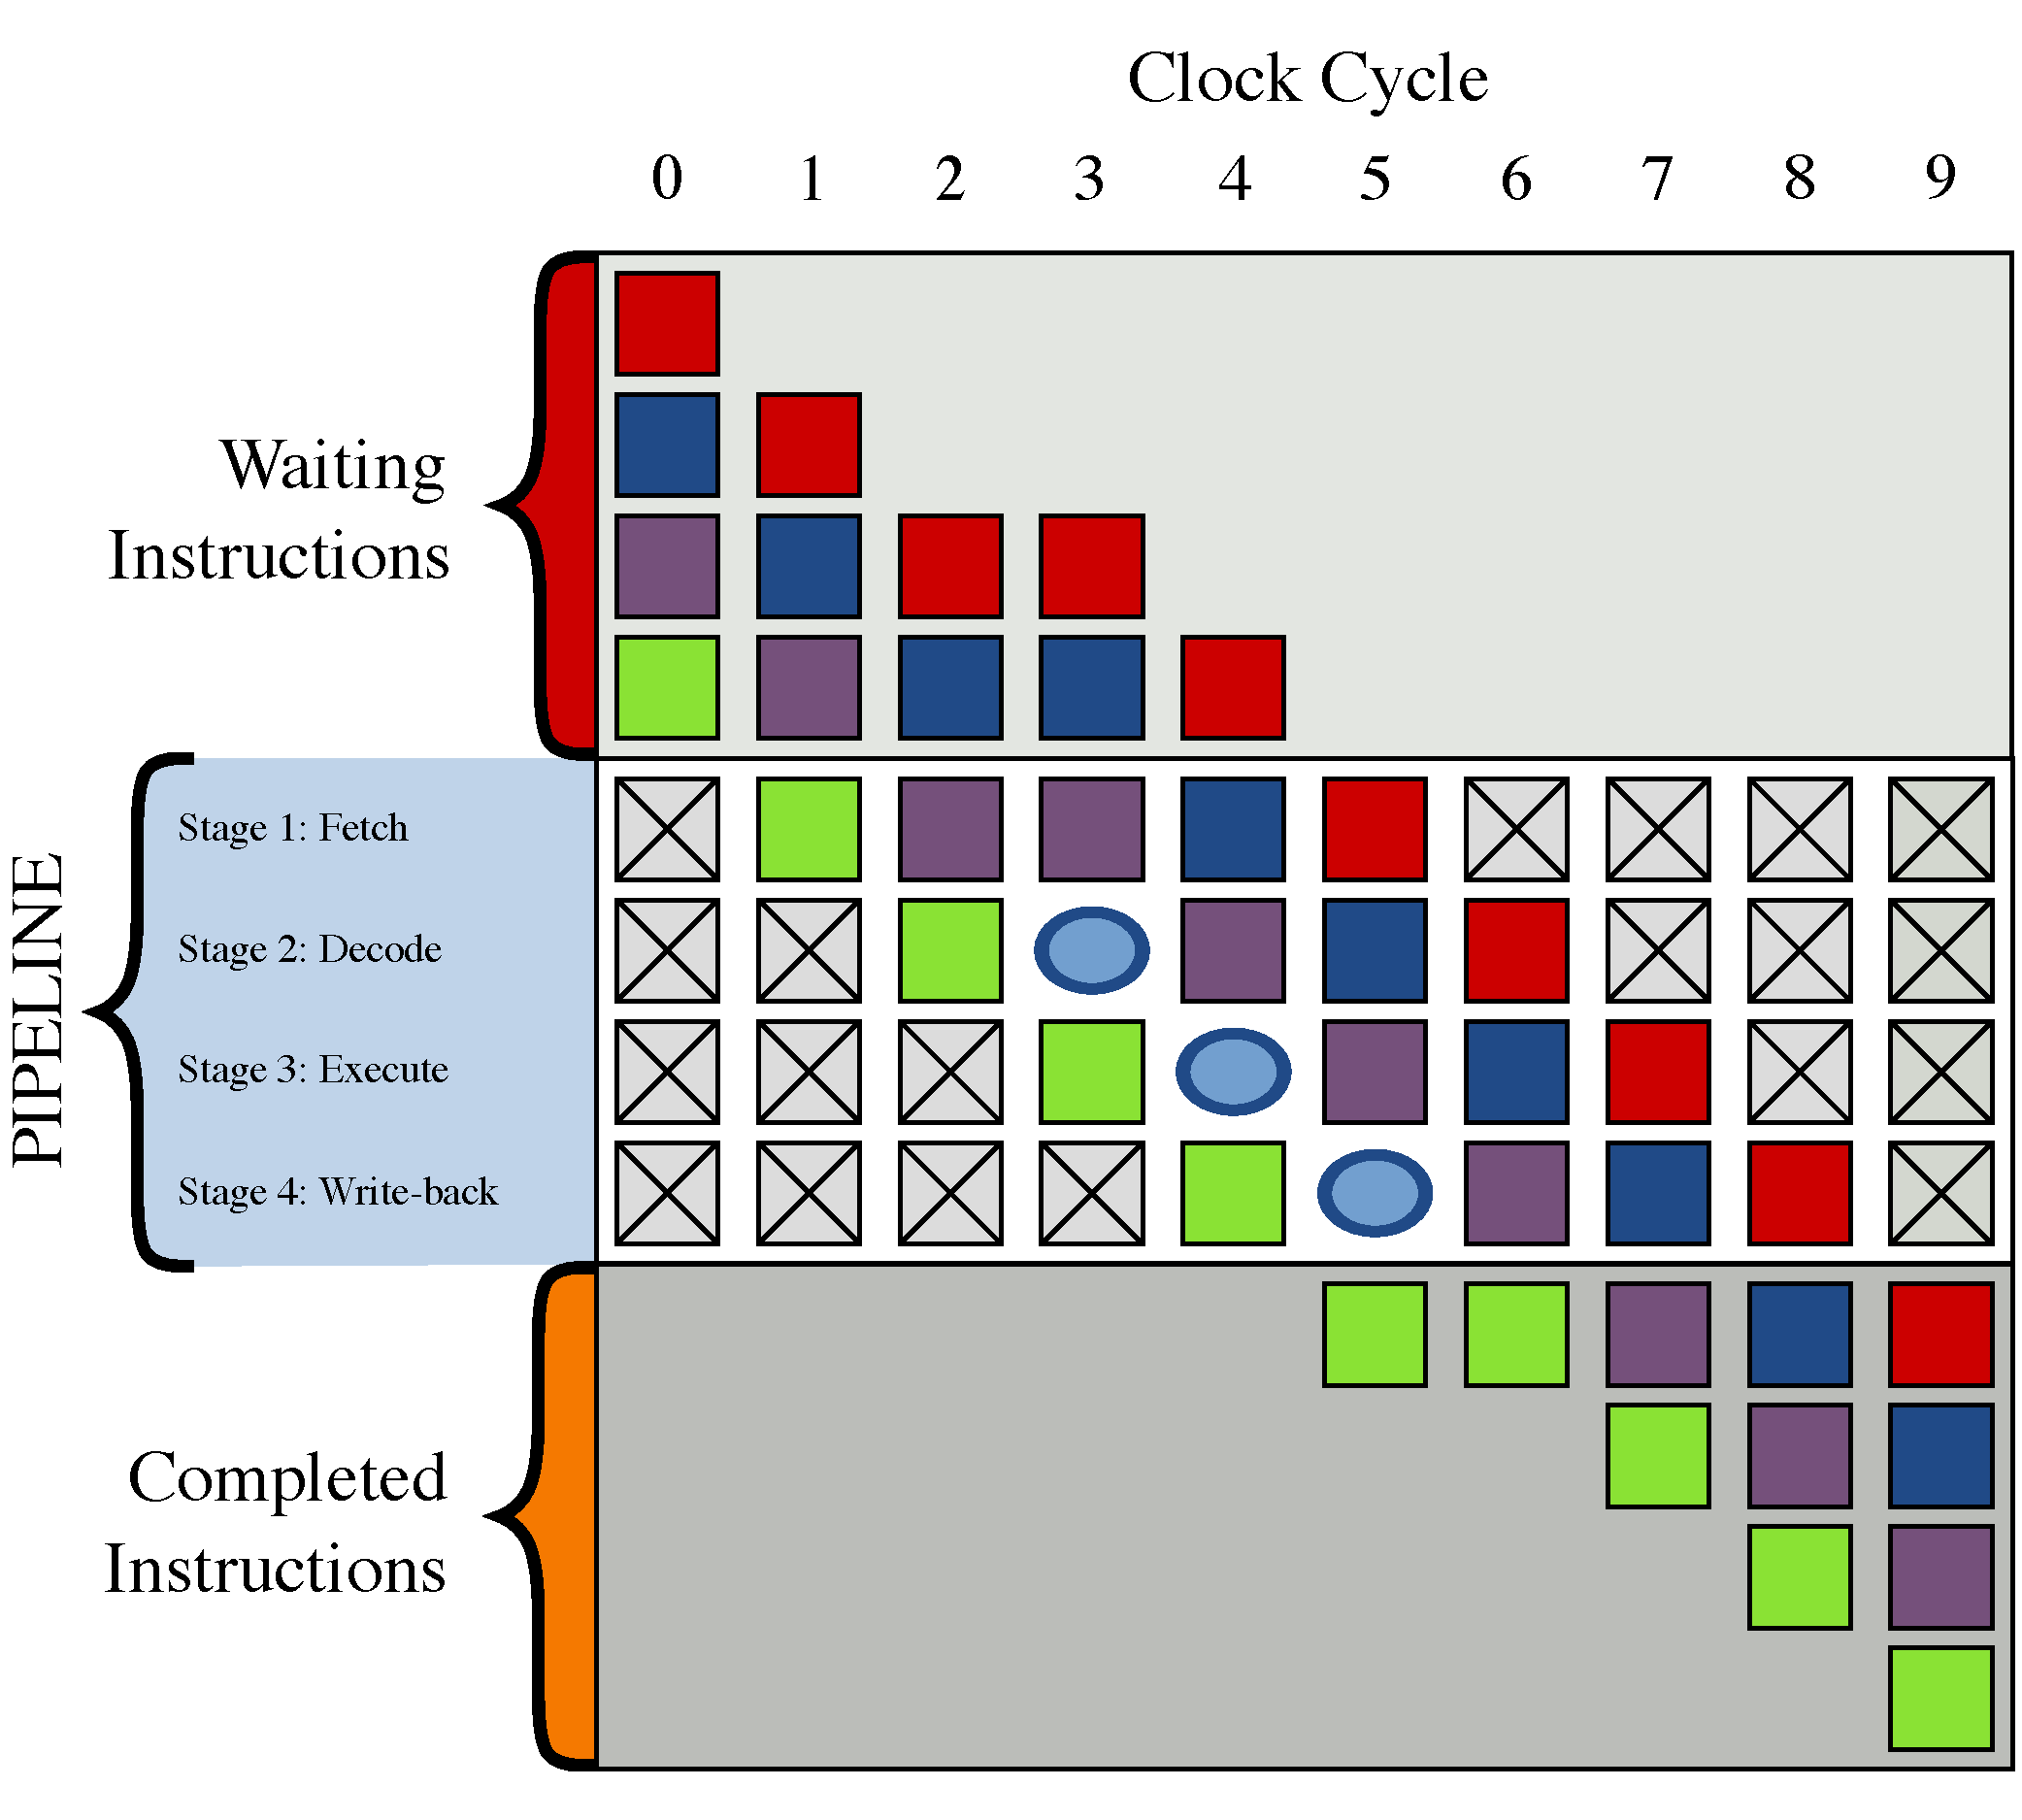
\includegraphics[width=1.0\linewidth]{images/7_pipeline/pipeline_4_stage_with_bubble.pdf}
			\caption{Esecuzione di una Pipeline in 4 stadi con una bolla}
			\label{fig:pipeline_4_stage_with_bubble}
		\end{figure}
	\end{columns}
	
\end{frame}


\subsubsection[Processori superscalari]{Processori superscalari}

\begin{frame}
	\frametitle{\textbullet{4} Pipeline}
	Per migliorare ulteriormente le prestazioni delle CPU sono state introdotti \textbf{processori superscalari}. In questi microprocessori vengono integrate più pipeline che funzionano in parallelo.
	
	%\begin{block}{Esecuzione fuori ordine}
		\begin{figure}[!htbp]
			\centering 
			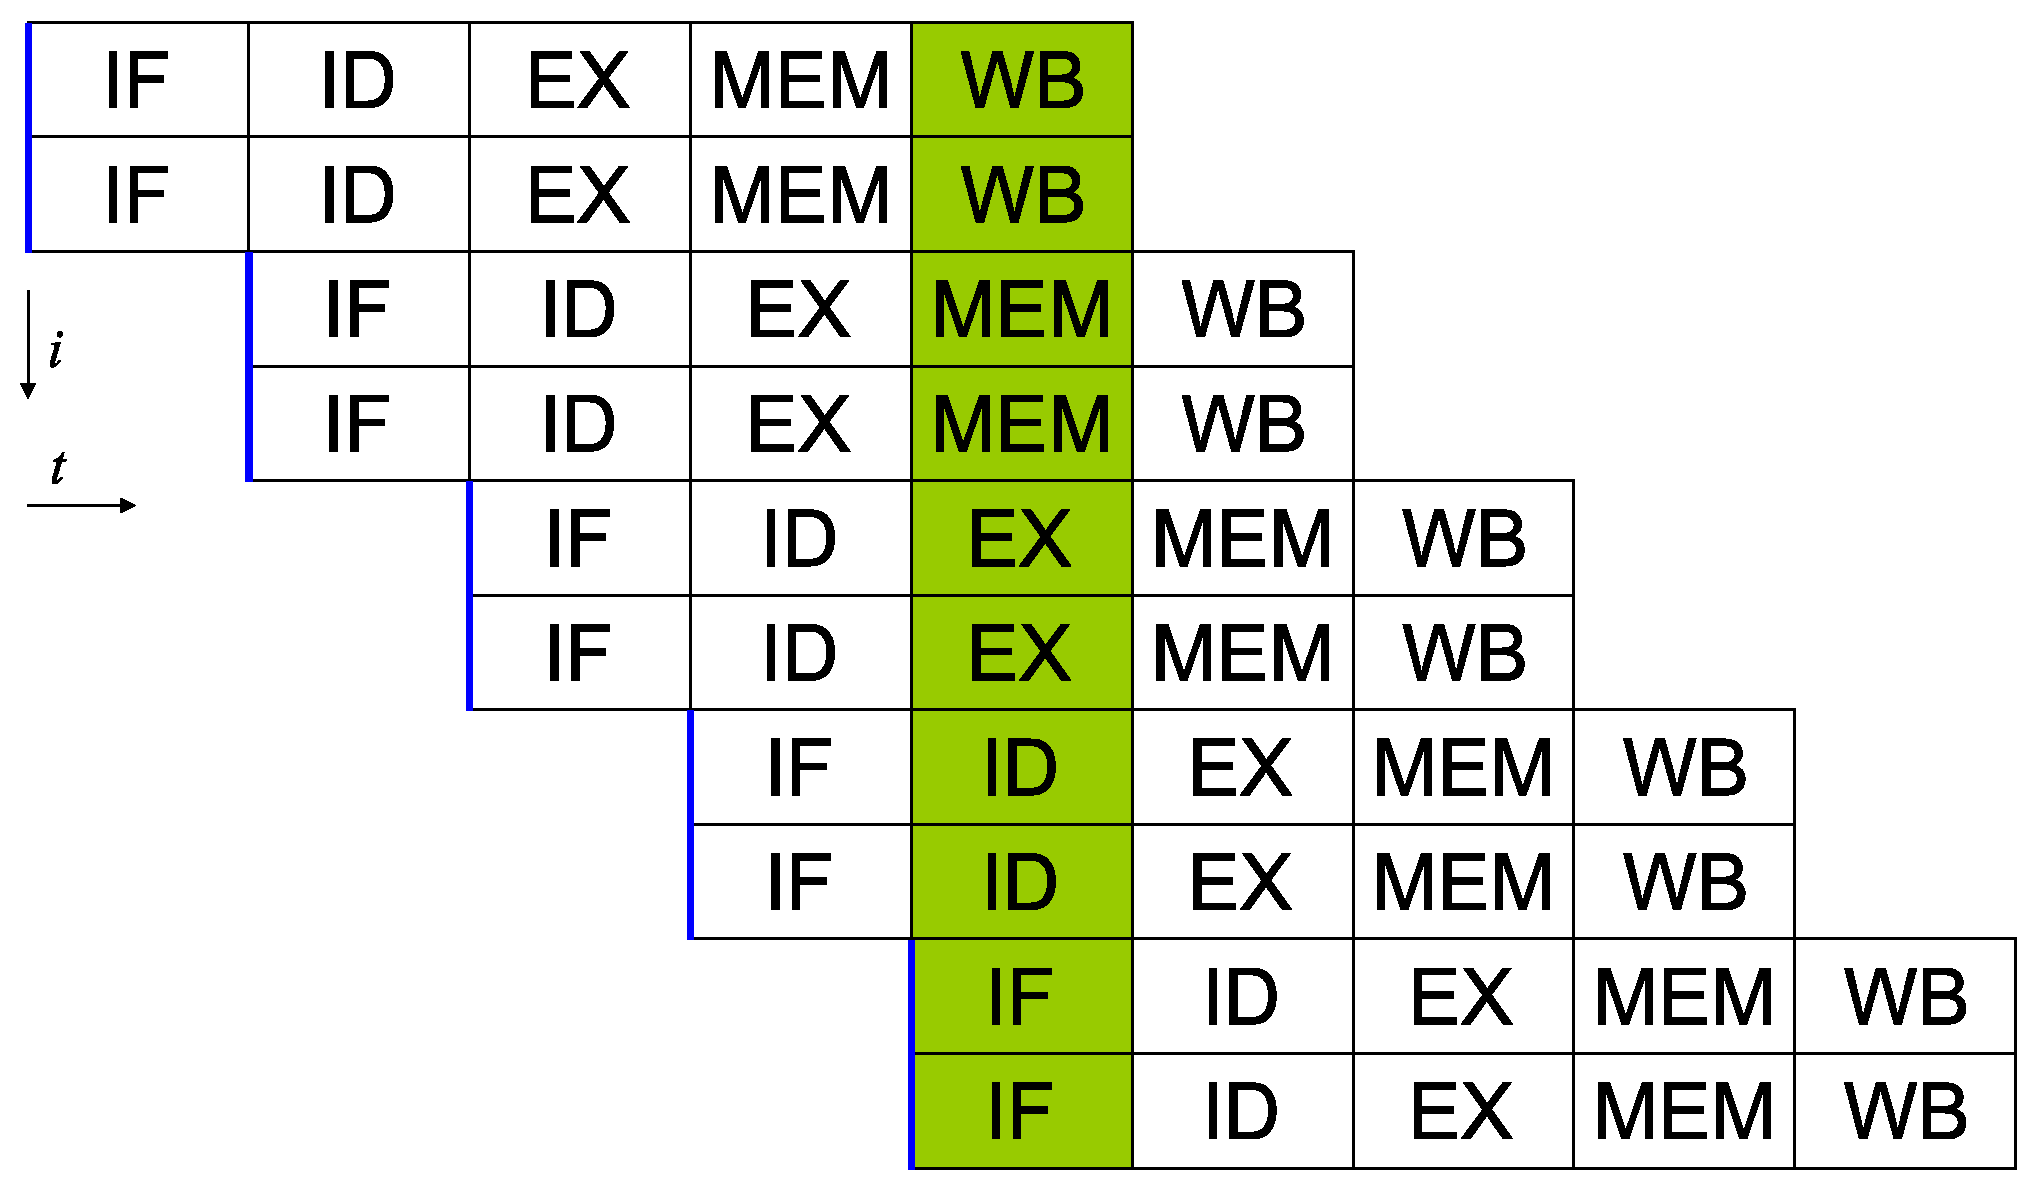
\includegraphics[width=0.7\linewidth]{images/7_pipeline/pipeline_superscalar.pdf}
			\caption{Una CPU superscalare}
			% (Microprocessor without Interlocked Pipelined Stages)
			\label{fig:pipeline_superscalar}
		\end{figure}
	%\end{block}

\end{frame}





\subsection[Cache memory]{Cache memory}
\begin{frame}
	\frametitle{\textbullet{5} Cache memory}
	
	%L'utilizzo di memorie cache, introduce una modifica al modello von Neumann, per migliorare le prestazioni complessive del sistema.
	\begin{block}{Le possibili modalità di gestione delle scritture nella cache:}
		\begin{itemize}
			\item \textbf{write through}: le scritture vengono propagate contemporaneamente in cache e memoria principale.
			\item \textbf{write back}: le scritture avvengono solo nella cache e poi sincronizzate con la memoria quando il blocco viene rimosso.
		\end{itemize}
		
	\end{block}


	\begin{block}{Gestione della Cache:}
		\begin{itemize}
			\item \textbf{metodo diretto}: ogni blocco è posizionato in una posizione specifica nella cache basata sull'indirizzo di memoria.
			\item \textbf{completamente associativo}: i blocchi possono essere collocati ovunque nella cache con la massima flessibilità.
			\item \textbf{associativo a N vie}: la cache è divisa in insiemi, ogni blocco può risiedere in uno solo dei N set ma all'interno del set è libero.% di occupare qualunque linea.
		\end{itemize}
		
	\end{block}
	
	
\end{frame}




\subsection[DMA (Direct Memory Access)]{DMA (Direct Memory Access)}
\begin{frame}
	\frametitle{\textbullet{6} DMA (Direct Memory Access)}
	
	\begin{block}{DMA (Direct Memory Access)}
		Nelle architetture non von Neumann, il DMA (Direct Memory Access) è una tecnica in cui un'unità specializzata gestisce il trasferimento diretto dei dati tra dispositivi esterni e la memoria, bypassando la CPU.\\~\\
		Ciò migliora l'efficienza, riducendo il carico sulla CPU e consentendo trasferimenti ad alta velocità, tipicamente utilizzati in periferiche come schede grafiche e dischi.\\~\\
		DMA accelera le operazioni di I/O poiché i dati sono trasferiti direttamente, senza passare attraverso il percorso tradizionale della CPU, ottimizzando il flusso di dati nell'architettura.
	\end{block}
	
\end{frame}


\begin{frame}
	\frametitle{\textbullet{6} DMA (Direct Memory Access)}
	
	\begin{figure}[!htbp]
		\centering 
		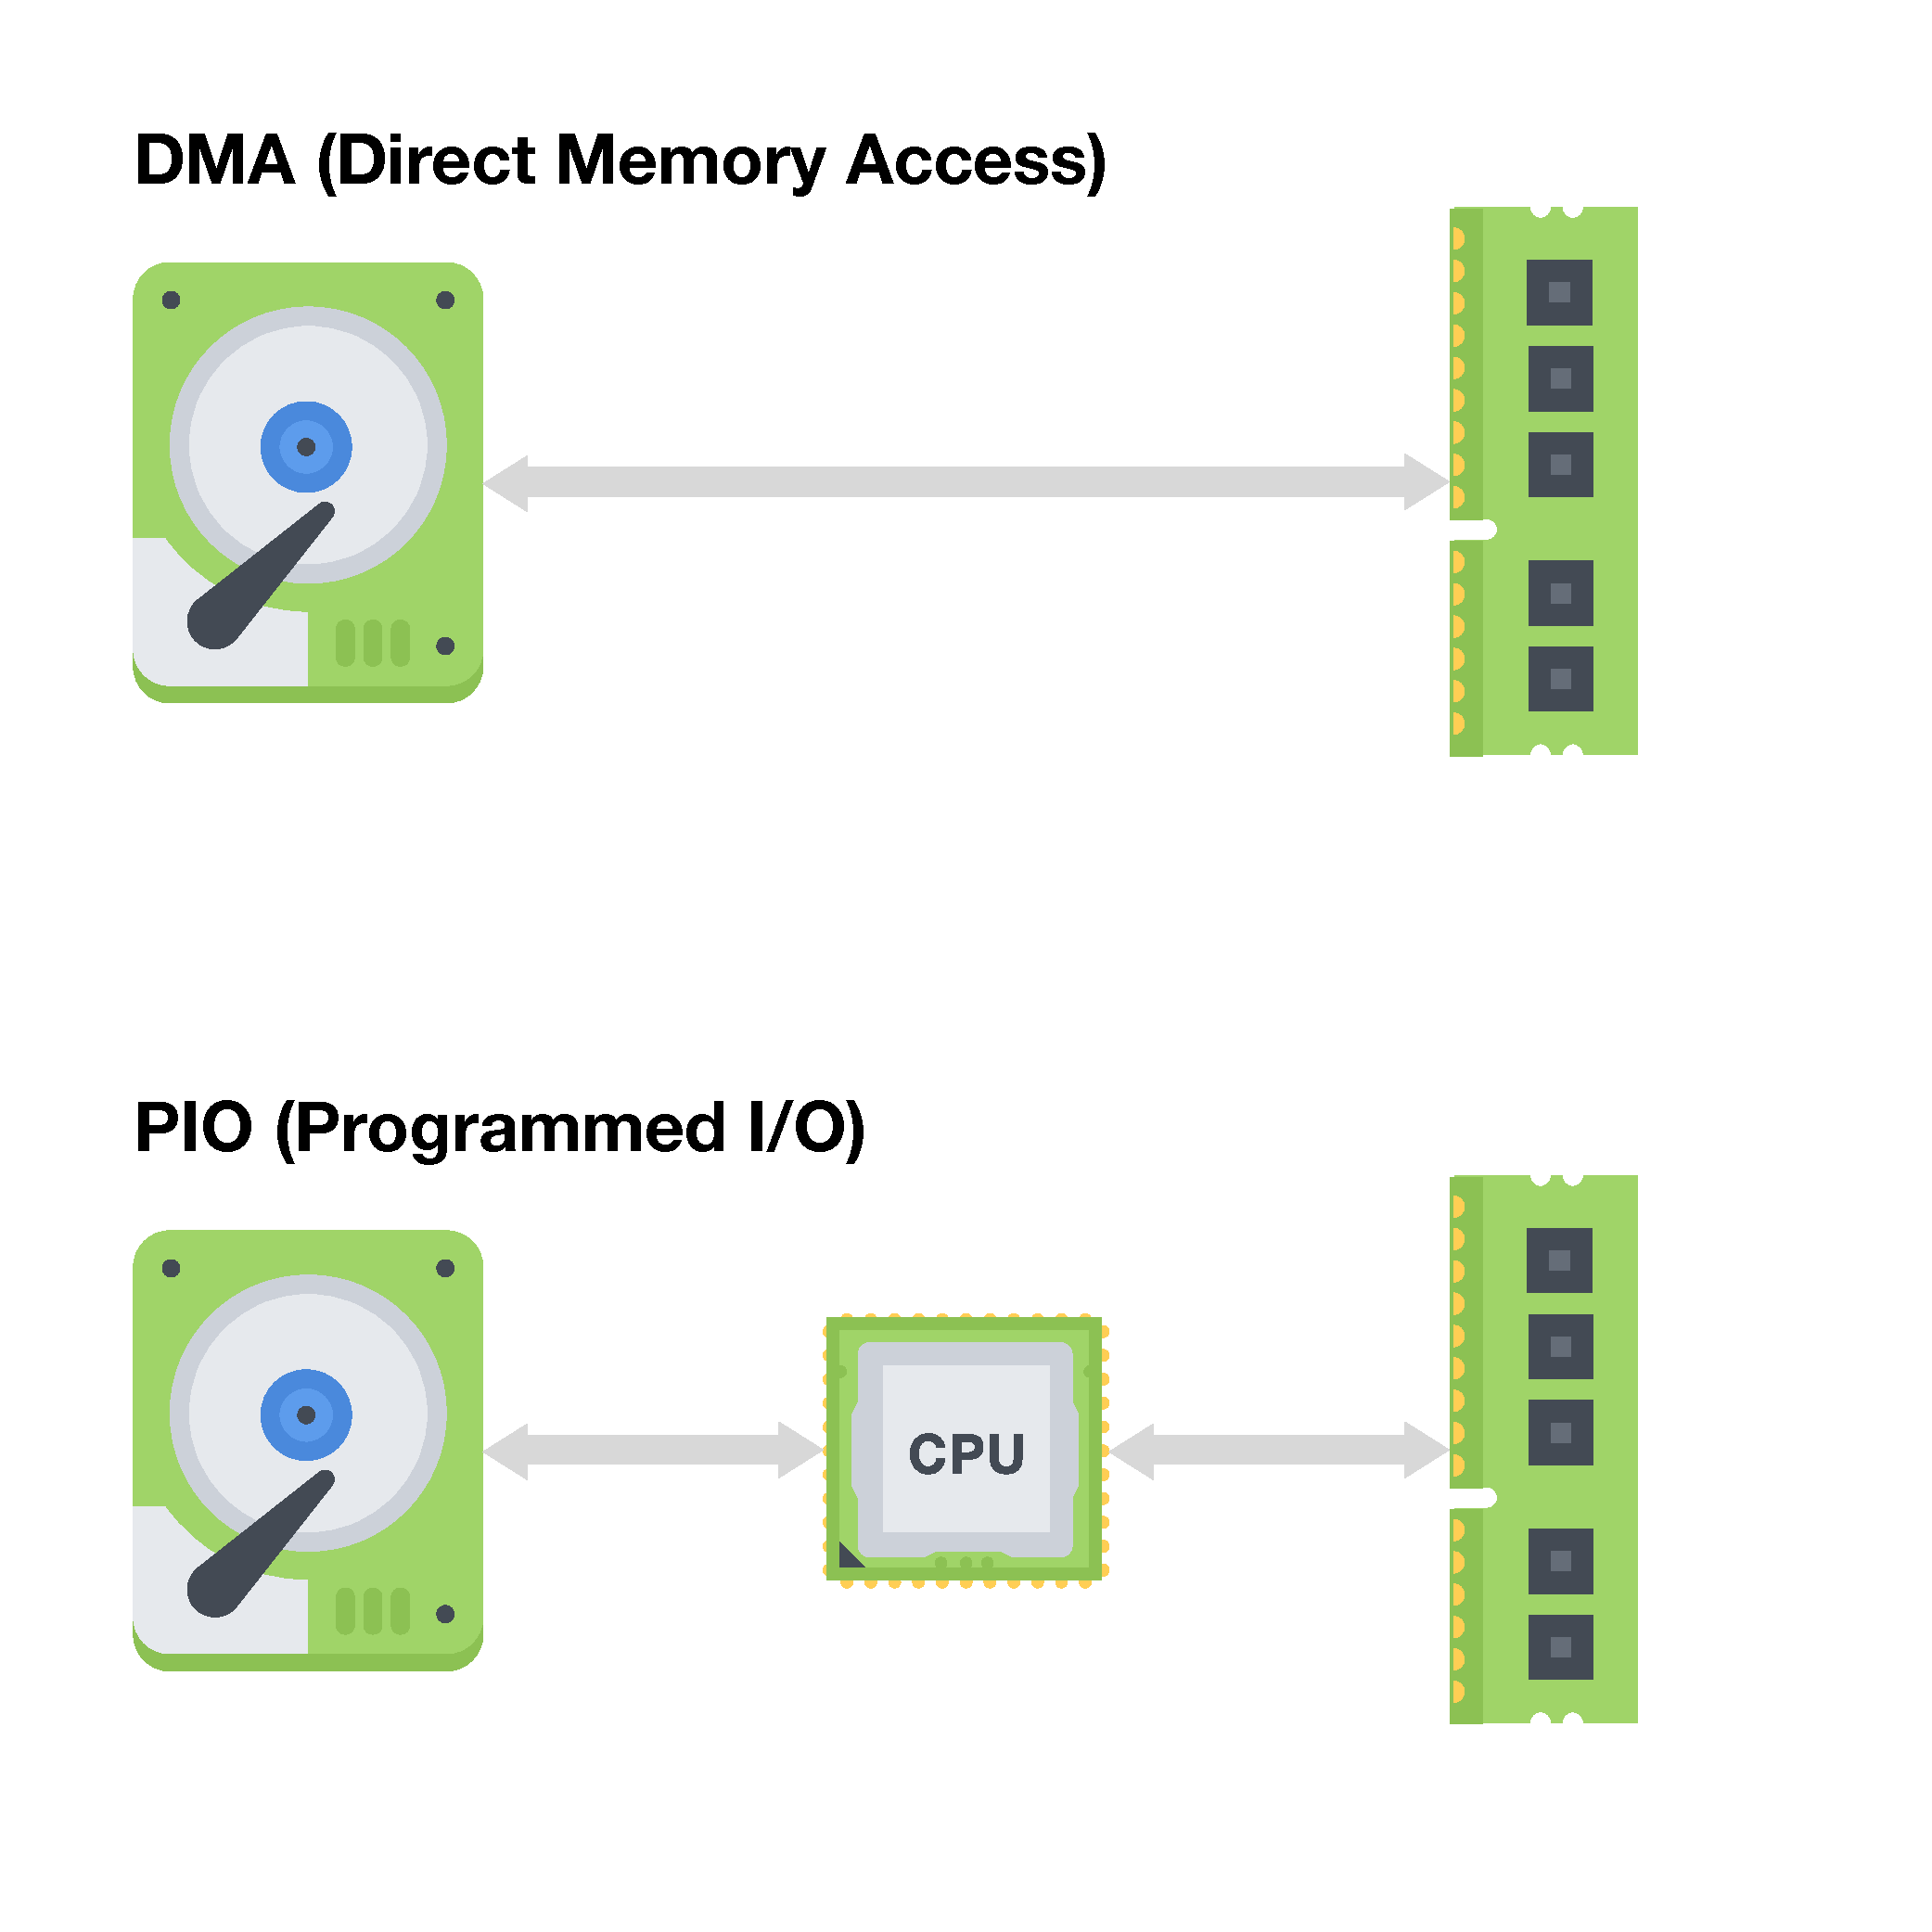
\includegraphics[width=0.6\linewidth]{images/7_pipeline/dma.pdf}
		%\caption{}
		%\label{}
	\end{figure}
\end{frame}




\subsection[Coprocessori]{Coprocessori}
\begin{frame}
	\frametitle{\textbullet{7} Coprocessori}
	
	\begin{block}{Coprocessori}
		I \textbf{coprocessori} sono unità specializzate che affiancano la CPU per eseguire operazioni specifiche:
		\begin{itemize}
			\item I \textbf{coprocessori numerici} si concentrano su calcoli matematici complessi, ad esempio calcoli in virgola mobile, migliorando le prestazioni computazionali. 
			\item I \textbf{coprocessori grafici (GPU)} sono dedicati al rendering grafico e all'elaborazione parallela, migliorando l'efficienza in contesti che utilizzano grafica avanzata e in applicazioni di intelligenza artificiale. 
		\end{itemize}
		
		La cooperazione tra coprocessori e CPU incrementa l'efficienza, consentendo l'esecuzione di compiti più veloci e complessi grazie a unità specializzate affiancate alla potenza di calcolo della CPU.
	\end{block}
	
\end{frame}


